% readme_flow.tex  the approach of the hopping-hare project in one row:
% model, master equation, two routes (deterministic and stochastic),
% comparison. Colours match build_chart.tex; section numbers refer to
% REPORT.md.
%
% Compile:  pdflatex readme_flow.tex     (or upload to Overleaf)
% PNG:      pdftoppm -png -r 220 -singlefile readme_flow.pdf readme_flow
\documentclass[border=8pt]{standalone}
\usepackage{amsmath}
\usepackage{tikz}
\usetikzlibrary{arrows.meta, positioning, calc}

\definecolor{ink}{HTML}{1F2937}
\definecolor{ink2}{HTML}{4B5563}
\definecolor{trunkfill}{HTML}{EEF4FB}
\definecolor{trunkline}{HTML}{2A78D6}
\definecolor{detfill}{HTML}{F3F4F6}
\definecolor{detline}{HTML}{4B5563}
\definecolor{luckfill}{HTML}{FDF1F5}
\definecolor{luckline}{HTML}{D6336C}
\definecolor{endfill}{HTML}{EEF8F1}
\definecolor{endline}{HTML}{2F855A}

\tikzset{
  box/.style = {rounded corners=4pt, line width=0.9pt, inner sep=7pt,
    align=left, text=ink, font=\normalsize,
    execute at begin node={\hyphenpenalty=10000\exhyphenpenalty=10000}},
  trunk/.style = {box, draw=trunkline, fill=trunkfill},
  det/.style = {box, draw=detline, fill=detfill},
  sto/.style = {box, draw=luckline, fill=luckfill},
  fin/.style = {box, draw=endline, fill=endfill},
  arrow/.style = {-{Stealth[length=3mm]}, line width=1pt, draw=ink2}
}
\newcommand{\ttl}[1]{{\large\bfseries #1}\par\smallskip}
\newcommand{\sub}[1]{{\itshape\color{ink2}#1}\par\smallskip}
\newcommand{\sect}[1]{\par\smallskip{\small\color{ink2}#1}}

\begin{document}
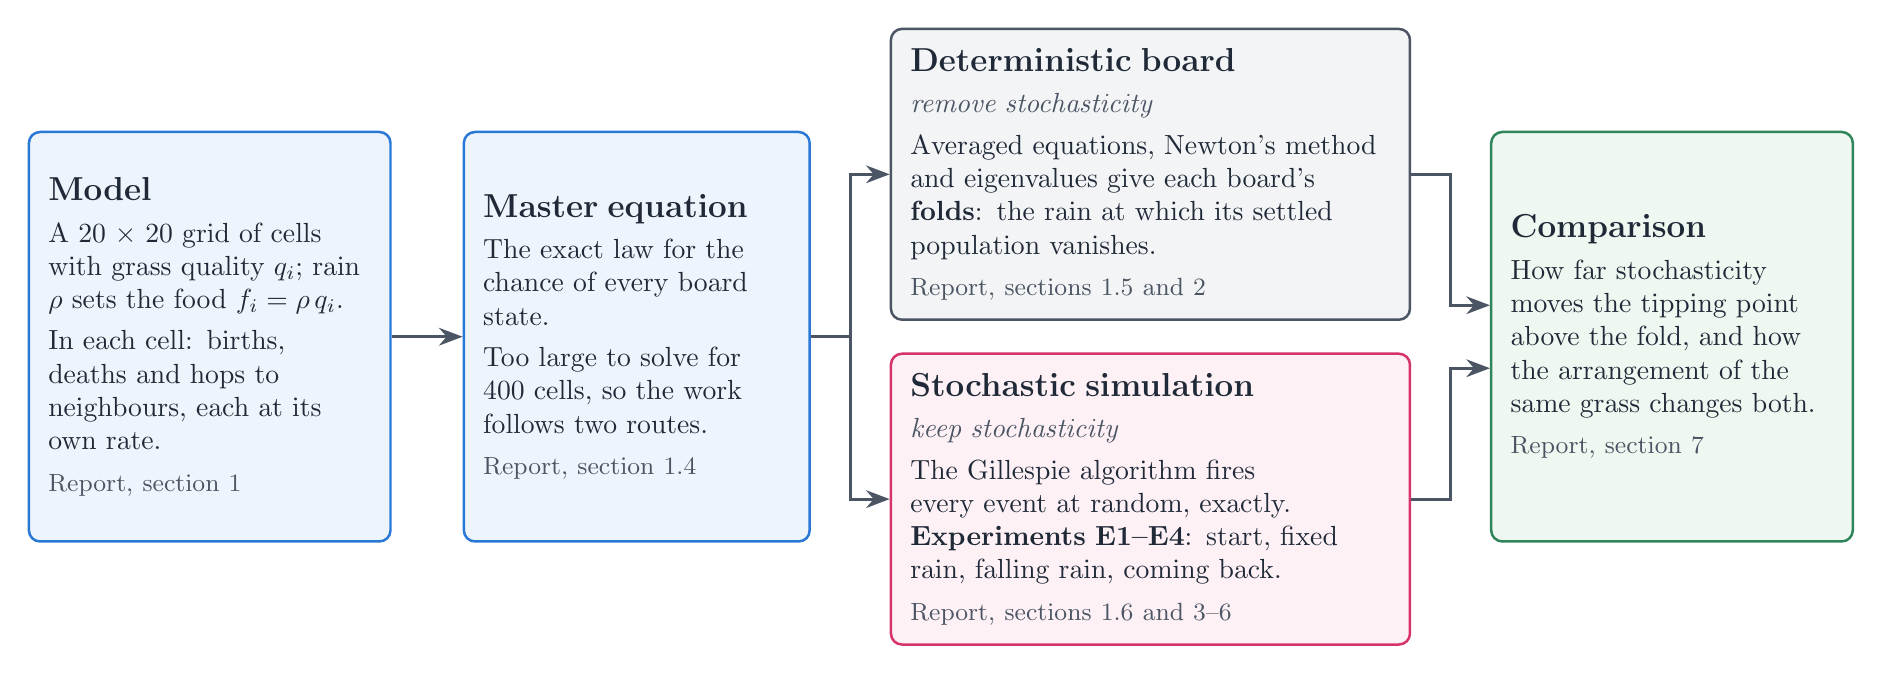
\begin{tikzpicture}

\node[trunk, text width=4.1cm, minimum height=5.2cm] (model) at (0, 0) {%
  \ttl{Model}
  A $20\times20$ grid of cells with grass quality $q_i$; rain $\rho$
  sets the food $f_i=\rho\,q_i$.\par\smallskip
  In each cell: births, deaths and hops to neighbours, each at its own
  rate.
  \sect{Report, section 1}};

\node[trunk, text width=3.9cm, minimum height=5.2cm,
      right=0.9cm of model] (master) {%
  \ttl{Master equation}
  The exact law for the chance of every board state.\par\smallskip
  Too large to solve for 400 cells, so the work follows two routes.
  \sect{Report, section 1.4}};

\node[det, text width=6.1cm, anchor=south west]
  (det) at ($(master.east)+(1.0, 0.2)$) {%
  \ttl{Deterministic board}
  \sub{remove stochasticity}
  Averaged equations, Newton's method and eigenvalues give each
  board's \textbf{folds}: the rain at which its settled population
  vanishes.
  \sect{Report, sections 1.5 and 2}};

\node[sto, text width=6.1cm, anchor=north west]
  (sto) at ($(master.east)+(1.0, -0.2)$) {%
  \ttl{Stochastic simulation}
  \sub{keep stochasticity}
  The Gillespie algorithm fires every event at random, exactly.
  \textbf{Experiments E1--E4}: start, fixed rain, falling rain, coming
  back.
  \sect{Report, sections 1.6 and 3--6}};

\node[fin, text width=4.1cm, minimum height=5.2cm,
      anchor=west] (cmp) at ($(det.east |- master.east)+(1.0, 0)$) {%
  \ttl{Comparison}
  How far stochasticity moves the tipping point above the fold, and how
  the arrangement of the same grass changes both.
  \sect{Report, section 7}};

\draw[arrow] (model) -- (master);
\draw[arrow] (master.east) -- ++(0.5, 0) |- (det.west);
\draw[arrow] (master.east) -- ++(0.5, 0) |- (sto.west);
\draw[arrow] (det.east) -- ++(0.5, 0) |- ($(cmp.west)+(0, 0.4)$);
\draw[arrow] (sto.east) -- ++(0.5, 0) |- ($(cmp.west)+(0, -0.4)$);

\end{tikzpicture}
\end{document}
